\documentclass[]{book}
\usepackage{lmodern}
\usepackage{amssymb,amsmath}
\usepackage{ifxetex,ifluatex}
\usepackage{fixltx2e} % provides \textsubscript
\ifnum 0\ifxetex 1\fi\ifluatex 1\fi=0 % if pdftex
  \usepackage[T1]{fontenc}
  \usepackage[utf8]{inputenc}
\else % if luatex or xelatex
  \ifxetex
    \usepackage{mathspec}
  \else
    \usepackage{fontspec}
  \fi
  \defaultfontfeatures{Ligatures=TeX,Scale=MatchLowercase}
\fi
% use upquote if available, for straight quotes in verbatim environments
\IfFileExists{upquote.sty}{\usepackage{upquote}}{}
% use microtype if available
\IfFileExists{microtype.sty}{%
\usepackage{microtype}
\UseMicrotypeSet[protrusion]{basicmath} % disable protrusion for tt fonts
}{}
\usepackage[margin=1in]{geometry}
\usepackage{hyperref}
\PassOptionsToPackage{usenames,dvipsnames}{color} % color is loaded by hyperref
\hypersetup{unicode=true,
            pdftitle={R Notes for Multivariate Analysis},
            pdfauthor={Yongfu, Liao},
            colorlinks=true,
            linkcolor=Maroon,
            citecolor=Blue,
            urlcolor=blue,
            breaklinks=true}
\urlstyle{same}  % don't use monospace font for urls
\usepackage{natbib}
\bibliographystyle{apalike}
\usepackage{color}
\usepackage{fancyvrb}
\newcommand{\VerbBar}{|}
\newcommand{\VERB}{\Verb[commandchars=\\\{\}]}
\DefineVerbatimEnvironment{Highlighting}{Verbatim}{commandchars=\\\{\}}
% Add ',fontsize=\small' for more characters per line
\usepackage{framed}
\definecolor{shadecolor}{RGB}{248,248,248}
\newenvironment{Shaded}{\begin{snugshade}}{\end{snugshade}}
\newcommand{\KeywordTok}[1]{\textcolor[rgb]{0.13,0.29,0.53}{\textbf{#1}}}
\newcommand{\DataTypeTok}[1]{\textcolor[rgb]{0.13,0.29,0.53}{#1}}
\newcommand{\DecValTok}[1]{\textcolor[rgb]{0.00,0.00,0.81}{#1}}
\newcommand{\BaseNTok}[1]{\textcolor[rgb]{0.00,0.00,0.81}{#1}}
\newcommand{\FloatTok}[1]{\textcolor[rgb]{0.00,0.00,0.81}{#1}}
\newcommand{\ConstantTok}[1]{\textcolor[rgb]{0.00,0.00,0.00}{#1}}
\newcommand{\CharTok}[1]{\textcolor[rgb]{0.31,0.60,0.02}{#1}}
\newcommand{\SpecialCharTok}[1]{\textcolor[rgb]{0.00,0.00,0.00}{#1}}
\newcommand{\StringTok}[1]{\textcolor[rgb]{0.31,0.60,0.02}{#1}}
\newcommand{\VerbatimStringTok}[1]{\textcolor[rgb]{0.31,0.60,0.02}{#1}}
\newcommand{\SpecialStringTok}[1]{\textcolor[rgb]{0.31,0.60,0.02}{#1}}
\newcommand{\ImportTok}[1]{#1}
\newcommand{\CommentTok}[1]{\textcolor[rgb]{0.56,0.35,0.01}{\textit{#1}}}
\newcommand{\DocumentationTok}[1]{\textcolor[rgb]{0.56,0.35,0.01}{\textbf{\textit{#1}}}}
\newcommand{\AnnotationTok}[1]{\textcolor[rgb]{0.56,0.35,0.01}{\textbf{\textit{#1}}}}
\newcommand{\CommentVarTok}[1]{\textcolor[rgb]{0.56,0.35,0.01}{\textbf{\textit{#1}}}}
\newcommand{\OtherTok}[1]{\textcolor[rgb]{0.56,0.35,0.01}{#1}}
\newcommand{\FunctionTok}[1]{\textcolor[rgb]{0.00,0.00,0.00}{#1}}
\newcommand{\VariableTok}[1]{\textcolor[rgb]{0.00,0.00,0.00}{#1}}
\newcommand{\ControlFlowTok}[1]{\textcolor[rgb]{0.13,0.29,0.53}{\textbf{#1}}}
\newcommand{\OperatorTok}[1]{\textcolor[rgb]{0.81,0.36,0.00}{\textbf{#1}}}
\newcommand{\BuiltInTok}[1]{#1}
\newcommand{\ExtensionTok}[1]{#1}
\newcommand{\PreprocessorTok}[1]{\textcolor[rgb]{0.56,0.35,0.01}{\textit{#1}}}
\newcommand{\AttributeTok}[1]{\textcolor[rgb]{0.77,0.63,0.00}{#1}}
\newcommand{\RegionMarkerTok}[1]{#1}
\newcommand{\InformationTok}[1]{\textcolor[rgb]{0.56,0.35,0.01}{\textbf{\textit{#1}}}}
\newcommand{\WarningTok}[1]{\textcolor[rgb]{0.56,0.35,0.01}{\textbf{\textit{#1}}}}
\newcommand{\AlertTok}[1]{\textcolor[rgb]{0.94,0.16,0.16}{#1}}
\newcommand{\ErrorTok}[1]{\textcolor[rgb]{0.64,0.00,0.00}{\textbf{#1}}}
\newcommand{\NormalTok}[1]{#1}
\usepackage{longtable,booktabs}
\usepackage{graphicx,grffile}
\makeatletter
\def\maxwidth{\ifdim\Gin@nat@width>\linewidth\linewidth\else\Gin@nat@width\fi}
\def\maxheight{\ifdim\Gin@nat@height>\textheight\textheight\else\Gin@nat@height\fi}
\makeatother
% Scale images if necessary, so that they will not overflow the page
% margins by default, and it is still possible to overwrite the defaults
% using explicit options in \includegraphics[width, height, ...]{}
\setkeys{Gin}{width=\maxwidth,height=\maxheight,keepaspectratio}
\IfFileExists{parskip.sty}{%
\usepackage{parskip}
}{% else
\setlength{\parindent}{0pt}
\setlength{\parskip}{6pt plus 2pt minus 1pt}
}
\setlength{\emergencystretch}{3em}  % prevent overfull lines
\providecommand{\tightlist}{%
  \setlength{\itemsep}{0pt}\setlength{\parskip}{0pt}}
\setcounter{secnumdepth}{5}
% Redefines (sub)paragraphs to behave more like sections
\ifx\paragraph\undefined\else
\let\oldparagraph\paragraph
\renewcommand{\paragraph}[1]{\oldparagraph{#1}\mbox{}}
\fi
\ifx\subparagraph\undefined\else
\let\oldsubparagraph\subparagraph
\renewcommand{\subparagraph}[1]{\oldsubparagraph{#1}\mbox{}}
\fi

%%% Use protect on footnotes to avoid problems with footnotes in titles
\let\rmarkdownfootnote\footnote%
\def\footnote{\protect\rmarkdownfootnote}

%%% Change title format to be more compact
\usepackage{titling}

% Create subtitle command for use in maketitle
\newcommand{\subtitle}[1]{
  \posttitle{
    \begin{center}\large#1\end{center}
    }
}

\setlength{\droptitle}{-2em}
  \title{R Notes for Multivariate Analysis}
  \pretitle{\vspace{\droptitle}\centering\huge}
  \posttitle{\par}
  \author{Yongfu, Liao}
  \preauthor{\centering\large\emph}
  \postauthor{\par}
  \predate{\centering\large\emph}
  \postdate{\par}
  \date{2018-04-06}

\usepackage{booktabs}

\usepackage{amsthm}
\newtheorem{theorem}{Theorem}[chapter]
\newtheorem{lemma}{Lemma}[chapter]
\theoremstyle{definition}
\newtheorem{definition}{Definition}[chapter]
\newtheorem{corollary}{Corollary}[chapter]
\newtheorem{proposition}{Proposition}[chapter]
\theoremstyle{definition}
\newtheorem{example}{Example}[chapter]
\theoremstyle{definition}
\newtheorem{exercise}{Exercise}[chapter]
\theoremstyle{remark}
\newtheorem*{remark}{Remark}
\newtheorem*{solution}{Solution}
\let\BeginKnitrBlock\begin \let\EndKnitrBlock\end
\begin{document}
\maketitle

{
\hypersetup{linkcolor=black}
\setcounter{tocdepth}{1}
\tableofcontents
}
\chapter*{About}\label{about}
\addcontentsline{toc}{chapter}{About}

This is a very simplified book about Multivariate Analysis in R. It is
written as a note to facilitate my learning of
\href{https://nol2.aca.ntu.edu.tw/nol/coursesearch/print_table.php?course_id=741\%20U3520\&class=\&dpt_code=7410\&ser_no=31954\&semester=106-2\&lang=CH}{Multivariate
Analysis at NTU}, Spring, 2018.

Feel free to share, modify, and reshare the work. For more information,
see the License section below.

\section*{License}\label{license}
\addcontentsline{toc}{section}{License}

This work is licensed under a
\href{https://creativecommons.org/licenses/by-nc/4.0/}{Creative Commons
Attribution-NonCommercial 4.0 International License}.

\chapter{Multivariate Normal Distribution \& Covariance
Matrix}\label{mvnorm}

\begin{Shaded}
\begin{Highlighting}[]
\KeywordTok{library}\NormalTok{(dplyr)}
\KeywordTok{library}\NormalTok{(latex2exp)}
\KeywordTok{library}\NormalTok{(ggplot2)}
\NormalTok{theme <-}\StringTok{ }\KeywordTok{theme}\NormalTok{(}\DataTypeTok{axis.text.x =} \KeywordTok{element_text}\NormalTok{(}\DataTypeTok{size =} \DecValTok{7}\NormalTok{, }\DataTypeTok{face =} \StringTok{"plain"}\NormalTok{, }\DataTypeTok{angle =} \DecValTok{30}\NormalTok{),}
               \DataTypeTok{axis.text.y =} \KeywordTok{element_text}\NormalTok{(}\DataTypeTok{size =} \DecValTok{7}\NormalTok{, }\DataTypeTok{face =} \StringTok{"plain"}\NormalTok{),}
               \DataTypeTok{axis.title.x =} \KeywordTok{element_text}\NormalTok{(}\DataTypeTok{size =} \DecValTok{9}\NormalTok{, }\DataTypeTok{face =} \StringTok{"bold"}\NormalTok{),}
    \DataTypeTok{axis.title.y =} \KeywordTok{element_text}\NormalTok{(}\DataTypeTok{size =} \DecValTok{9}\NormalTok{, }\DataTypeTok{face =} \StringTok{"bold"}\NormalTok{))}
\end{Highlighting}
\end{Shaded}

\section{Bivariate Normal Contour
Map}\label{bivariate-normal-contour-map}

\subsection{\texorpdfstring{\texttt{ellipse}
function}{ellipse function}}\label{ellipse-function}

\begin{Shaded}
\begin{Highlighting}[]
\KeywordTok{ellipse}\NormalTok{(x, scale, centre, level, }\DataTypeTok{npoints =} \DecValTok{1000}\NormalTok{)}
\end{Highlighting}
\end{Shaded}

\begin{itemize}
\item
  \texttt{x}: a single number, correlation of the two variables.
\item
  \texttt{scale}: vector, \textbf{standard deviation} of the two
  variables.
\item
  \texttt{centre}: vector, center of the ellipse, i.e.~the mean vector
  of the bivariate normal distribution.
\item
  \texttt{level}: a single number, the contour probability.
\item
  \texttt{npoints}: number of points used to draw the contour.
\end{itemize}

\texttt{ellipse} returns a \textbf{matrix} with dimension
(\texttt{npoints} \(\times\) 2), which can be used to plot contour.

\subsection{Data Generation}\label{data-generation}

The \texttt{for} loop below is used to generate a data frame with 3
columns(variables):

\begin{itemize}
\item
  Column 1: First variable of bivariate normal function (\(x_1\))
\item
  Column 2: Second variable of bivariate normal function (\(x_2\))
\item
  Column 3: The contour that \(x_1\) \& \(x_2\) on the same row belongs
  to.
\end{itemize}

\begin{Shaded}
\begin{Highlighting}[]
\KeywordTok{library}\NormalTok{(ellipse)}

\NormalTok{All_contours <-}\StringTok{ }\KeywordTok{c}\NormalTok{(}\OtherTok{NA}\NormalTok{, }\OtherTok{NA}\NormalTok{, }\OtherTok{NA}\NormalTok{) }
\NormalTok{    ## Set empty start for appending ##}

\ControlFlowTok{for}\NormalTok{ (i }\ControlFlowTok{in} \DecValTok{1}\OperatorTok{:}\DecValTok{5}\NormalTok{) \{}
\NormalTok{    level <-}\StringTok{ }\FloatTok{0.1}\OperatorTok{*}\NormalTok{i }
\NormalTok{        ## Set Contour prob., prob. of obs within contour ##}
\NormalTok{    ell_data <-}\KeywordTok{ellipse}\NormalTok{(}\OperatorTok{-}\FloatTok{0.8}\NormalTok{, }\KeywordTok{c}\NormalTok{(}\KeywordTok{sqrt}\NormalTok{(}\DecValTok{2}\NormalTok{), }\DecValTok{1}\NormalTok{), }\DataTypeTok{centre =} \KeywordTok{c}\NormalTok{(}\DecValTok{1}\NormalTok{, }\DecValTok{3}\NormalTok{), }\DataTypeTok{level =}\NormalTok{ level, }\DataTypeTok{npoints =} \DecValTok{800}\OperatorTok{+}\NormalTok{(i}\OperatorTok{-}\DecValTok{1}\NormalTok{)}\OperatorTok{^}\DecValTok{3}\NormalTok{)}
\NormalTok{        ## npoints: bigger contours with more points ##}
\NormalTok{    class <-}\StringTok{ }\KeywordTok{rep}\NormalTok{(}\KeywordTok{paste}\NormalTok{(level}\OperatorTok{*}\DecValTok{100}\NormalTok{, }\StringTok{"% Contour"}\NormalTok{, }\DataTypeTok{sep=}\StringTok{""}\NormalTok{), }\KeywordTok{nrow}\NormalTok{(ell_data))}
\NormalTok{        ## Assign contour class ##}
\NormalTok{    ell_data <-}\StringTok{ }\KeywordTok{as.data.frame}\NormalTok{(ell_data)}
\NormalTok{        ## Change to data.frame BEFORE cbind, ##}
\NormalTok{        ## or coersion happens ##}
\NormalTok{    ell_data <-}\StringTok{ }\KeywordTok{cbind}\NormalTok{(ell_data, class)}
    
\NormalTok{    All_contours <-}\StringTok{ }\KeywordTok{rbind}\NormalTok{(All_contours, ell_data)}
\NormalTok{\}}

\NormalTok{All_contours <-}\StringTok{ }\NormalTok{All_contours[}\OperatorTok{-}\DecValTok{1}\NormalTok{,]}
\NormalTok{    ## Remove the empty start ##}
\end{Highlighting}
\end{Shaded}

\subsection{Plotting}\label{plotting}

\begin{Shaded}
\begin{Highlighting}[]
\KeywordTok{ggplot}\NormalTok{(}\DataTypeTok{data =}\NormalTok{ All_contours) }\OperatorTok{+}
\StringTok{    }\KeywordTok{geom_point}\NormalTok{(}\KeywordTok{aes}\NormalTok{(}\DataTypeTok{x =}\NormalTok{ x, }\DataTypeTok{y =}\NormalTok{ y, }\DataTypeTok{color =}\NormalTok{ class),}
               \DataTypeTok{size =} \FloatTok{0.1}\NormalTok{) }\OperatorTok{+}
\StringTok{    }\KeywordTok{scale_colour_grey}\NormalTok{(}\DataTypeTok{start =} \FloatTok{0.7}\NormalTok{, }\DataTypeTok{end =} \FloatTok{0.3}\NormalTok{) }\OperatorTok{+}
\StringTok{        }\NormalTok{## Use gray scales instead of colored default ##}
\StringTok{    }\KeywordTok{labs}\NormalTok{(}\DataTypeTok{color =} \StringTok{"Contours"}\NormalTok{, }
         \DataTypeTok{title =} \StringTok{"Contour Plot"}\NormalTok{,}
         \DataTypeTok{x =} \KeywordTok{TeX}\NormalTok{(}\StringTok{"$x_1$"}\NormalTok{), }\DataTypeTok{y =} \KeywordTok{TeX}\NormalTok{(}\StringTok{"$x_2$"}\NormalTok{)}
\NormalTok{    )}
\end{Highlighting}
\end{Shaded}

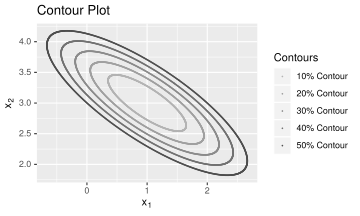
\includegraphics{Notes_files/figure-latex/unnamed-chunk-3-1.pdf}

\section{Multivariate Normal
Functions}\label{multivariate-normal-functions}

\subsection{Generate density f(x)}\label{generate-density-fx}

\begin{Shaded}
\begin{Highlighting}[]
\KeywordTok{library}\NormalTok{(mvtnorm)}

\NormalTok{mu <-}\StringTok{ }\KeywordTok{c}\NormalTok{(}\DecValTok{1}\NormalTok{, }\DecValTok{3}\NormalTok{) }\CommentTok{# mean vector}
\NormalTok{Sigma <-}\StringTok{ }\KeywordTok{matrix}\NormalTok{(}\KeywordTok{c}\NormalTok{(}\DecValTok{2}\NormalTok{, }\OperatorTok{-}\FloatTok{0.8}\OperatorTok{*}\KeywordTok{sqrt}\NormalTok{(}\DecValTok{2}\NormalTok{), }\OperatorTok{-}\FloatTok{0.8}\OperatorTok{*}\KeywordTok{sqrt}\NormalTok{(}\DecValTok{2}\NormalTok{), }\DecValTok{1}\NormalTok{),}
                \DataTypeTok{nrow =} \DecValTok{2}\NormalTok{) }\CommentTok{# covariance matrix}

\KeywordTok{dmvnorm}\NormalTok{(}\DataTypeTok{x =} \KeywordTok{c}\NormalTok{(}\DecValTok{2}\NormalTok{, }\DecValTok{5}\NormalTok{), }\DataTypeTok{mean =}\NormalTok{ mu, }\DataTypeTok{sigma =}\NormalTok{ Sigma)}
\end{Highlighting}
\end{Shaded}

\begin{verbatim}
[1] 1.562995e-05
\end{verbatim}

\begin{itemize}
\tightlist
\item
  \texttt{x}: Vector x in f(x), all variables of the multivariate normal
  distribution.
\item
  \texttt{mean}: Mean vector(center of ellipse) of the multivariate
  normal distribution.
\item
  \texttt{sigma}: Covariance matrix of the multivariate normal
  distribution.
\end{itemize}

\texttt{dmvnorm} returns f(x), the range of the multivariate normal
function. For example,
\texttt{dmvnorm(x\ =\ c(2,\ 5),\ mean\ =\ mu,\ sigma\ =\ Sigma)} returns
the value f(\(x_1=2\), \(x_2=5\)) of the multivariate normal
distribution specified by mean vector, \texttt{mu}, and covariance
matrix, \texttt{Sigma}.

\subsubsection{Example: Densities of a
Contour}\label{example-densities-of-a-contour}

\begin{Shaded}
\begin{Highlighting}[]
\NormalTok{data <-}\StringTok{ }\NormalTok{All_contours }\OperatorTok\StringTok{ }
\StringTok{    }\KeywordTok{filter}\NormalTok{(class }\OperatorTok{==}\StringTok{ "50% Contour"}\NormalTok{)}

\KeywordTok{dmvnorm}\NormalTok{(}\DataTypeTok{x =}\NormalTok{ data[}\DecValTok{1}\NormalTok{, }\DecValTok{1}\OperatorTok{:}\DecValTok{2}\NormalTok{], }\DataTypeTok{mean =}\NormalTok{ mu, }\DataTypeTok{sigma =}\NormalTok{ Sigma)[[}\DecValTok{1}\NormalTok{]]}
\end{Highlighting}
\end{Shaded}

\begin{verbatim}
[1] 0.09378295
\end{verbatim}

\begin{Shaded}
\begin{Highlighting}[]
\KeywordTok{dmvnorm}\NormalTok{(}\DataTypeTok{x =}\NormalTok{ data[}\DecValTok{4}\NormalTok{, }\DecValTok{1}\OperatorTok{:}\DecValTok{2}\NormalTok{], }\DataTypeTok{mean =}\NormalTok{ mu, }\DataTypeTok{sigma =}\NormalTok{ Sigma)[[}\DecValTok{1}\NormalTok{]]}
\end{Highlighting}
\end{Shaded}

\begin{verbatim}
[1] 0.09378295
\end{verbatim}

The retured values are the same(very close), since they are on the same
contour. See the section \protect\hypertarget{data-generation}{}{above}
for more details.

\subsection{Covariance Matrix}\label{covariance-matrix}

Generater covariance and correlation Matricies:

\begin{Shaded}
\begin{Highlighting}[]
\KeywordTok{library}\NormalTok{(mat2tex)}
\NormalTok{cov.mt <-}\StringTok{ }\KeywordTok{cov}\NormalTok{(iris[,}\DecValTok{1}\OperatorTok{:}\DecValTok{4}\NormalTok{]) ## Cov Matrix of variable 1~4}
\NormalTok{cor.mt <-}\StringTok{ }\KeywordTok{cor}\NormalTok{(iris[,}\DecValTok{1}\OperatorTok{:}\DecValTok{4}\NormalTok{]) ## Cor Matrix of variable 1~4}
\end{Highlighting}
\end{Shaded}

Covariance matrix
\(= \begin{pmatrix}  0.69 & -0.04 & 1.27 & 0.52 \\  -0.04 & 0.19 & -0.33 & -0.12 \\  1.27 & -0.33 & 3.12 & 1.30 \\  0.52 & -0.12 & 1.30 & 0.58 \\  \end{pmatrix}\)

Correlation matrix
\(= \begin{pmatrix}  1.00 & -0.12 & 0.87 & 0.82 \\  -0.12 & 1.00 & -0.43 & -0.37 \\  0.87 & -0.43 & 1.00 & 0.96 \\  0.82 & -0.37 & 0.96 & 1.00 \\  \end{pmatrix}\)

\chapter{Principle Component Analysis}\label{PCA}

\section{Workflow of PCA}\label{workflow-of-pca}

\hypertarget{conceptual}{\subsection{Conceptual}\label{conceptual}}

\hypertarget{htmlwidget-709c1f636273545a16de}{}

\subsection{Computational (with R)}\label{computational-with-r}

\hypertarget{htmlwidget-2f0307270d976e9e74e1}{}

\begin{itemize}
\tightlist
\item
  Note: \texttt{sdev} of \texttt{prcomp()} are \textbf{Standard
  Deviations}. To get the eigenvalues of the covariance (correlation)
  matrix, or equivalently, variances of the principle components, you
  need to \textbf{square \texttt{sdev}}.
\end{itemize}

\section{Conversion Between Correlation \& Covaraince
Matrices}\label{conversion-between-correlation-covaraince-matrices}

\subsection{\texorpdfstring{\texttt{prcomp()}}{prcomp()}}\label{prcomp}

The function \texttt{prcomp()} in base R \texttt{stats} package performs
principle component analysis to input \texttt{data.frame}(with
observations as rows and variables as columns), but it returns neither
covariance nor correlation matrix. You can compute them directly by
passing \texttt{data.frame} to \texttt{cor()} and \texttt{cov()}
directly in R without any additional package.

\BeginKnitrBlock{bs-callout bs-callout-warning}
{prcomp() vs.~princomp()}

There is another function, \texttt{princomp()}, in \texttt{stats} that
performs PCA. This function is based on spectral decomposition\footnote{The
  Conceptual workflow of PCA at Section
  \protect\hyperlink{conceptual}{2.1.1} is based on spectral
  decomposition.} while \texttt{prcomp()} is based on SVD\footnote{You
  can check the answers at
  \href{https://stats.stackexchange.com/questions/20101/what-is-the-difference-between-r-functions-prcomp-and-princomp}{Stack
  Overflow}}. SVD has greater numeric accuracy, so \texttt{prcomp()} is
preferred.
\EndKnitrBlock{bs-callout bs-callout-warning}

\subsection{Covariance to Correlation}\label{covariance-to-correlation}

Sometimes there is no raw data but only covariance or correlation
matrix, and you may want to convert one to another. This can be done by
using simple matrix multiplication, based on the fact that

\[\mathbf{R} = diag(\mathbf{S})^{\frac{-1}{2}} ~ \mathbf{S} ~ diag(\mathbf{S})^{\frac{-1}{2}}
\label{eq:cov2cor}\]

, where \(\mathbf{R}\) is the correlation matrix, \(\mathbf{S}\) is the
covariance matrix, and \(diag(\mathbf{S})\) is the diagonal matrix
composed of diagonal elements of \(\mathbf{S}\).

\subsection{\texorpdfstring{\texttt{eigen()}}{eigen()}}\label{eigen}

After obtaining the covariance or correlation matrix, direct computation
of eigenvalue and eigenvectors is straightforward: pass the matrix to
base R \texttt{eigen()} function.

\begin{Shaded}
\begin{Highlighting}[]
\KeywordTok{cov}\NormalTok{(iris[,}\DecValTok{1}\OperatorTok{:}\DecValTok{3}\NormalTok{]) }\OperatorTok\StringTok{ }\KeywordTok{eigen}\NormalTok{()}
\end{Highlighting}
\end{Shaded}

\begin{verbatim}
eigen() decomposition
$values
[1] 3.69111979 0.24137727 0.05945372

$vectors
            [,1]       [,2]       [,3]
[1,]  0.38983343  0.6392233 -0.6628903
[2,] -0.09100801  0.7430587  0.6630093
[3,]  0.91637735 -0.1981349  0.3478435
\end{verbatim}

\section{Scree Plot}\label{scree-plot}

Scree plot is an important tool for determining the importance of
principle components. Although the logic of plotting scree plots is
easy, it may be quite annoying for repeating the code every time.

\subsection{\texorpdfstring{\texttt{screeplot()} from Base
R}{screeplot() from Base R}}\label{screeplot-from-base-r}

There is a ready-written function for scree plot in \texttt{stats}
package, but the output is terrible:

\begin{Shaded}
\begin{Highlighting}[]
\KeywordTok{prcomp}\NormalTok{(iris[,}\DecValTok{1}\OperatorTok{:}\DecValTok{3}\NormalTok{]) }\OperatorTok\StringTok{ }\KeywordTok{screeplot}\NormalTok{(}\DataTypeTok{type=}\StringTok{"lines"}\NormalTok{)}
\end{Highlighting}
\end{Shaded}

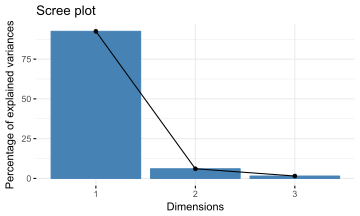
\includegraphics{Notes_files/figure-latex/unnamed-chunk-13-1.pdf}

\subsection{\texorpdfstring{\texttt{fviz\_eig()} from
\texttt{factoextra}}{fviz\_eig() from factoextra}}\label{fviz_eig-from-factoextra}

For a better-looking scree plot function, I recommend
\texttt{fviz\_eig()} from \texttt{factoextra} \citep{R-factoextra}.
\texttt{fviz\_eig()} has better looking outputs and more customizable
plotting parameters, and since it is based on \texttt{ggplot2}, you can
actually enhance it with the \texttt{ggplot2} syntax: \texttt{+}.

\begin{Shaded}
\begin{Highlighting}[]
\KeywordTok{library}\NormalTok{(factoextra)}
\KeywordTok{prcomp}\NormalTok{(iris[,}\DecValTok{1}\OperatorTok{:}\DecValTok{3}\NormalTok{]) }\OperatorTok\StringTok{ }\KeywordTok{fviz_eig}\NormalTok{()}
\end{Highlighting}
\end{Shaded}

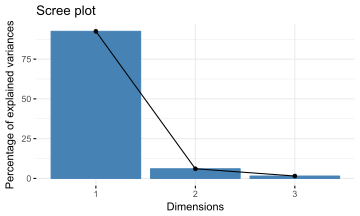
\includegraphics{Notes_files/figure-latex/unnamed-chunk-14-1.pdf}

\begin{Shaded}
\begin{Highlighting}[]
\KeywordTok{prcomp}\NormalTok{(iris[,}\DecValTok{1}\OperatorTok{:}\DecValTok{3}\NormalTok{]) }\OperatorTok\StringTok{ }
\StringTok{    }\KeywordTok{fviz_eig}\NormalTok{(}\DataTypeTok{choice =} \StringTok{"eigenvalue"}\NormalTok{, }\CommentTok{# y as eigenvalue}
             \DataTypeTok{geom =} \StringTok{"line"}\NormalTok{,}
             \DataTypeTok{addlabels =}\NormalTok{ T) }\OperatorTok{+}
\StringTok{    }\KeywordTok{scale_y_continuous}\NormalTok{(}\DataTypeTok{limits =} \KeywordTok{c}\NormalTok{(}\DecValTok{0}\NormalTok{, }\DecValTok{5}\NormalTok{))}
\end{Highlighting}
\end{Shaded}

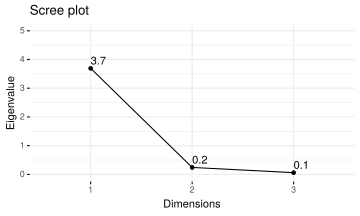
\includegraphics{Notes_files/figure-latex/unnamed-chunk-15-1.pdf}

\subsection{Customized Function}\label{customized-function}

I have OCD with plotting, so not completely satisfied with
\texttt{factoextra::fviz\_eig()}. So I created my own
\texttt{scree\_plot()} by building on \texttt{fviz\_eig()}\footnote{Check
  \href{https://github.com/liao961120/local_depend/blob/master/R\%20functions/multivariate_fc.R}{\texttt{multivariate\_fc.R}},
  starting at line 46.}, which supports \textbf{double y-axis}: one
showing eigenvalue, the other proportion of total variance explained.

\section{Q-Q Plot}\label{q-q-plot}

Q-Q plots are for checking the normality assumuption and are also useful
for detecting outlyers. Principle components are linear combinations of
the original variables, so if the original variables come from a
multivariate normal distribution, principle components are expected to
have normal distributions.

\subsection{\texorpdfstring{\texttt{qqnorm()} from Base
R}{qqnorm() from Base R}}\label{qqnorm-from-base-r}

There is also a base R \texttt{qqnorm()} function, which plots sample
quantiles against theoretical quantiles obtain from the standard normal
distribution.

\begin{Shaded}
\begin{Highlighting}[]
\KeywordTok{prcomp}\NormalTok{(iris[}\DecValTok{1}\OperatorTok{:}\DecValTok{60}\NormalTok{, }\DecValTok{1}\OperatorTok{:}\DecValTok{3}\NormalTok{])[[}\StringTok{"x"}\NormalTok{]][,}\DecValTok{1}\NormalTok{] }\OperatorTok\StringTok{ }
\StringTok{    }\KeywordTok{qqnorm}\NormalTok{()}
\end{Highlighting}
\end{Shaded}

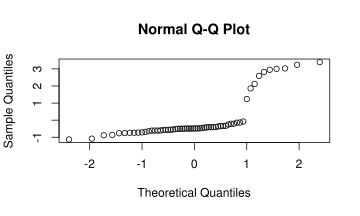
\includegraphics{Notes_files/figure-latex/unnamed-chunk-16-1.pdf}

\texttt{prcomp(data.frame){[}{[}"x"{]}{]}} returns the principle
component scores, i.e.~data that are \textbf{rotated} or
\textbf{weighted} by the elements of the eigenvectors.

\texttt{prcomp(data.frame){[}{[}"x"{]}{]}{[},1{]}} subsets the first
column of the principle component scores, which is the scores of the
First principle component, i.e.~data weighted according to elements of
the first (corresponding to the largest eigenvalue) eigenvector.

\subsection{Self-defined Function}\label{self-defined-function}

\texttt{qqnorm()} is pretty good but lacks one important feature:
\textbf{labeling points on the Q-Q plot so that identification of the
points is possible}.

So I wrote my own function \texttt{QQplot}, which labels every point on
the graph:

\begin{Shaded}
\begin{Highlighting}[]
\NormalTok{QQplot <-}\StringTok{ }\ControlFlowTok{function}\NormalTok{(x, }\DataTypeTok{ID=}\StringTok{"none"}\NormalTok{, }
                   \DataTypeTok{theme=}\OtherTok{NULL}\NormalTok{, }\DataTypeTok{color=}\StringTok{"red"}\NormalTok{, }\DataTypeTok{text=}\OtherTok{TRUE}\NormalTok{,}
                   \DataTypeTok{text_adj=}
                       \KeywordTok{c}\NormalTok{(}\DataTypeTok{hjust=}\OperatorTok{-}\FloatTok{0.1}\NormalTok{, }\DataTypeTok{vjust=}\DecValTok{0}\NormalTok{, }\DataTypeTok{size=}\DecValTok{3}\NormalTok{)) \{}
    \KeywordTok{library}\NormalTok{(dplyr)}
    \KeywordTok{library}\NormalTok{(ggplot2)}
    
\NormalTok{    x <-}\StringTok{ }\KeywordTok{as_data_frame}\NormalTok{(x) }
\NormalTok{    n <-}\StringTok{ }\KeywordTok{nrow}\NormalTok{(x)}
\NormalTok{    quantiles <-}\StringTok{ }\KeywordTok{qnorm}\NormalTok{(}\DataTypeTok{p=}\KeywordTok{seq}\NormalTok{(}\FloatTok{0.5}\OperatorTok{/}\NormalTok{n, }\DecValTok{1}\OperatorTok{-}\FloatTok{0.5}\OperatorTok{/}\NormalTok{n, }\DecValTok{1}\OperatorTok{/}\NormalTok{n))}
    
    \ControlFlowTok{if}\NormalTok{ (ID }\OperatorTok{==}\StringTok{ "none"}\NormalTok{) \{ }\CommentTok{# assign ID if not passed}
\NormalTok{        ID <-}\StringTok{ }\KeywordTok{as.character}\NormalTok{(}\DecValTok{1}\OperatorTok{:}\NormalTok{n)}
\NormalTok{    \} }\ControlFlowTok{else}\NormalTok{ \{}
\NormalTok{        ID <-}\StringTok{ }\KeywordTok{as_data_frame}\NormalTok{(ID)}
\NormalTok{        ID <-}\StringTok{ }\KeywordTok{as.character}\NormalTok{(ID[[}\KeywordTok{colnames}\NormalTok{(ID)]])}
\NormalTok{        \}}
    
    \ControlFlowTok{if}\NormalTok{ (text }\OperatorTok{==}\StringTok{ }\OtherTok{TRUE}\NormalTok{) \{}
\NormalTok{        text <-}\StringTok{ }\KeywordTok{geom_text}\NormalTok{(}\KeywordTok{aes}\NormalTok{(}\DataTypeTok{label=}\NormalTok{ID),}
                              \DataTypeTok{hjust=}\NormalTok{text_adj[}\DecValTok{1}\NormalTok{],}
                              \DataTypeTok{vjust=}\NormalTok{text_adj[}\DecValTok{2}\NormalTok{],}
                              \DataTypeTok{size =}\NormalTok{ text_adj[}\DecValTok{3}\NormalTok{])}
\NormalTok{    \} }\ControlFlowTok{else}\NormalTok{ \{text <-}\StringTok{ }\OtherTok{NULL}\NormalTok{\}}
    
\NormalTok{    data <-}\StringTok{ }\KeywordTok{cbind}\NormalTok{(ID, x)}
    \KeywordTok{colnames}\NormalTok{(data) <-}\StringTok{ }\KeywordTok{c}\NormalTok{(}\StringTok{"ID"}\NormalTok{, }\StringTok{"x"}\NormalTok{)}
\NormalTok{    data <-}\StringTok{ }\NormalTok{data }\OperatorTok\StringTok{ }\KeywordTok{arrange}\NormalTok{(x) }\OperatorTok\StringTok{ }\KeywordTok{mutate}\NormalTok{(}\DataTypeTok{quantile=}\NormalTok{quantiles)}
    
\NormalTok{    pl <-}\StringTok{ }\KeywordTok{ggplot}\NormalTok{(data, }\KeywordTok{aes}\NormalTok{(}\DataTypeTok{x=}\NormalTok{quantiles, }\DataTypeTok{y=}\NormalTok{x))}\OperatorTok{+}
\StringTok{        }\KeywordTok{geom_point}\NormalTok{(}\DataTypeTok{color=}\NormalTok{color)}\OperatorTok{+}
\StringTok{        }\NormalTok{text }\OperatorTok{+}\StringTok{ }\NormalTok{theme }\OperatorTok{+}
\StringTok{        }\KeywordTok{labs}\NormalTok{(}\DataTypeTok{x=}\StringTok{"Theoretical Quantile"}\NormalTok{,}
             \DataTypeTok{y=}\StringTok{"x"}\NormalTok{,}
             \DataTypeTok{title=}\StringTok{"Q-Q Plot"}\NormalTok{)}
\NormalTok{    pl}
\NormalTok{\}}
\end{Highlighting}
\end{Shaded}

\begin{Shaded}
\begin{Highlighting}[]
\KeywordTok{prcomp}\NormalTok{(iris[}\DecValTok{1}\OperatorTok{:}\DecValTok{60}\NormalTok{, }\DecValTok{1}\OperatorTok{:}\DecValTok{3}\NormalTok{])[[}\StringTok{"x"}\NormalTok{]][,}\DecValTok{1}\NormalTok{] }\OperatorTok
\StringTok{    }\KeywordTok{QQplot}\NormalTok{()}
\end{Highlighting}
\end{Shaded}

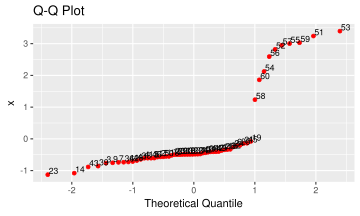
\includegraphics{Notes_files/figure-latex/unnamed-chunk-18-1.pdf}

\bibliography{book.bib,packages.bib}


\end{document}
